
\subsection{Using Rolled Up Factor Graphs}
\label{sec:rolledUpFactorGraphs}


\subsubsection{Markov Model}

In our first rolled up graph we build a simple Markov model describing an infinite stream of variables.   

\ifmatlab

\begin{lstlisting}
%%%%%%%%%%%%%%%%%%%%%%%%%%%%%%%%%                                                                                             
%Markov Model                                                                                                                 
%%%%%%%%%%%%%%%%%%%%%%%%%%%%%%%%%                                                                                             

%%%%%%%%%%%%%%%%%%%%%%%%%%%%%%%%%                                                                                             
%Build nested graph                                                                                                           
%%%%%%%%%%%%%%%%%%%%%%%%%%%%%%%%%                                                                                             

%Here we build a graph that connects two variables by an xor 
%equation An xor equation with only two variables is the 
%equivalent of an equals constraint.                                                                                                 

in = Bit();
out = Bit();
ng = FactorGraph(in,out);
ng.addFactor(@xorDelta,in,out);


%%%%%%%%%%%%%%%%%%%%%%%%%%%%%%%%%                                                                                             
%create rolled up graph.                                                                                                      
%%%%%%%%%%%%%%%%%%%%%%%%%%%%%%%%%                                                                                             

%Now we build a FactorGraph that creates an infinite chain of %variables.                                                     
bs = BitStream();
fg = FactorGraph();

%Passing variable streams as arguments to addFactor will result 
%in a rolled up graph.  Passing in a slice of a variable stream 
%specifies a relative offset for where the nested graph should 
%be connected to the variable stream.                       
fs = fg.addFactor(ng,bs,bs.getSlice(2));

%%%%%%%%%%%%%%%%%%%%%%%%%%%%%%%%%                                                                                             
%create data source                                                                                                           
%%%%%%%%%%%%%%%%%%%%%%%%%%%%%%%%%  
data = repmat([.4 .6]',1,10);
ds = DoubleArrayDataSource(data);
dsink = DoubleArrayDataSink();
bs.DataSource = ds;
bs.DataSink = dsink;

%%%%%%%%%%%%%%%%%%%%%%%%%%%%%%%%%                                                                                             
%solve 
%%%%%%%%%%%%%%%%%%%%%%%%%%%%%%%%%                                                                                             
fg.solve();

%%%%%%%%%%%%%%%%%%%%%%%%%%%%%%%%%                                                                                             
%get Beliefs
%%%%%%%%%%%%%%%%%%%%%%%%%%%%%%%%%                                                                                             
while dsink.hasNext()
    dsink.getNext()
end

\end{lstlisting}

\fi

\ifjava
\begin{lstlisting}
/////////////////////////////////                                                                                             
//Markov Model                                                                                                                 
/////////////////////////////////

/////////////////////////////////                                                                                             
//Build nested graph                                                                                                           
/////////////////////////////////                                                                                             

//Here we build a graph that connects two variables by an xor 
//equation An xor equation with only two variables is the 
//equivalent of an equals constraint.                                                                                                 
Equals eq = new Equals();
Bit in = new Bit();
Bit out = new Bit();
FactorGraph ng = new FactorGraph(in,out);
ng.addFactor(eq,in,out);


/////////////////////////////////                                                                                             
//create rolled up graph.                                                                                                      
/////////////////////////////////                                                                                             

//Now we build a FactorGraph that creates an infinite chain of %variables.                                                     
BitStream bs = new BitStream();
FactorGraph fg = new FactorGraph();


//Passing variable streams as arguments to addFactor will result 
//in a rolled up graph.  Passing in a slice of a variable stream 
//specifies a relative offset for where the nested graph should 
//be connected to the variable stream.                       
FactorGraphStream fs = fg.addRepeatedFactor(ng,bs,bs.getSlice(2));

/////////////////////////////////                                                                                             
//create data source                                                                                                           
/////////////////////////////////
double [][] data = new double[10][];
for (int i = 0; i < 10; i++)
	data[i] = new double [] {0.4,0.6};
		
DoubleArrayDataSource ds = new DoubleArrayDataSource(data);
DoubleArrayDataSink dsink = new DoubleArrayDataSink();
bs.setDataSource(ds);
bs.setDataSink(dsink);

/////////////////////////////////                                                                                             
//solve 
/////////////////////////////////                                                                                             
fg.solve();

/////////////////////////////////                                                                                             
//get Beliefs
/////////////////////////////////
while (dsink.hasNext())
	System.out.println(Arrays.toString(dsink.getNext()));
\end{lstlisting}
\fi


Let's talk about some of the aspects of rolled up graphs illustrated in this example in more detail:

\para{Variable Streams and Slices}

Variable Streams represent infinite streams of variables.  When instantiating a VariableStream, users have to specify a domain.  The following are examples of instantiating Discrete VariableStreams:

\ifmatlab
\begin{itemize}
\item DiscreteStream(DiscreteDomain($\{$0,1,2$\}$));
\item DiscreteStream($\{$0,1,2$\}$); - equivalent to the previous example
\item DiscreteStream($\{$0,1$\}$); - A stream of bits
\item BitStream(); - Shorthand for the previous example.
\end{itemize}
\fi

\ifjava
\begin{itemize}
\item new DiscreteStream(new DiscreteDomain(0,1,2));
\item DiscreteStream(0,1,2); - equivalent to the previous example
\item new DiscreteStream(0,1); - A stream of bits
\item new BitStream(); - Shorthand for the previous example.
\end{itemize}
\fi

\ifmatlab

Users can optionally create streams of vectors of variables.  When doing so, users have to specify the dimensions of their variables

\begin{itemize}
\item DiscreteStream([0 1 2],N,1) - For a column vector
\item DiscreteStream([0 1 2],1,N) - For a row vector
\item DiscreteStream([0 1 2],M,N,P) - For a three dimensional tensor
\end{itemize}

\fi

When adding a repeated FactorGraph, users need to be able to specify how a nested graph connects to the variable streams.  Slices can be used to indicate where in the stream a nested graph should connect.  Slices are essentially references to a Variable Stream with a specified offset and increment.  Slices have two main methods:

\begin{itemize}
\item hasNext() -- Returns true if the next variable referenced by the slice can be retrieved.
\item getNext() -- Returns the next variable in the  slice if it can be referenced.  Otherwise throws an error.
\end{itemize}

Users typically shouldn't use these methods.  Slices should primarily be used as arguments to addFactor.

First we need to instantiate a variable stream:

\ifmatlab
\begin{lstlisting}
S = BitStream();
\end{lstlisting}
\fi

\ifjava
\begin{lstlisting}
BitStream S = new BitStream();
\end{lstlisting}
\fi


We can get slices in the following way:

\begin{itemize}

\item S.getSlice(start); -- Start specifies this slices starting point as an index into the variable stream.
\end{itemize}

\para{Buffer Size}

Users can specify a bufferSize for each FactorGraph stream.  A FactorGraphStream is instantiated every time addFactor is called with a nestedGraph and VariableStreams or Slices.  The default bufferSize is 1.  Solving a graph with bufferSize one will result in a forward only algorithm.  The bufferSize indicates how many nested graphs to instantiate for one step.  In our Markov Model example, when buffer size is set to 1 and we plot the graph before solving we see this:

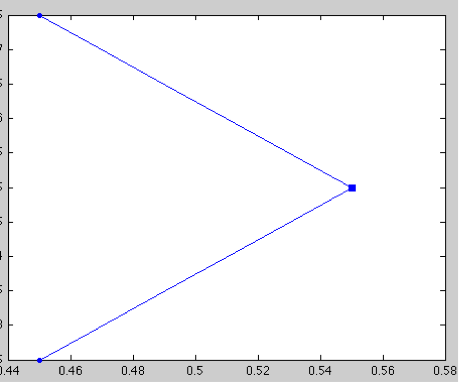
\includegraphics{images/BufferSize1.png}

We see one factor and two instantiated variables.  If we set bufferSize to 5 and plot we get:

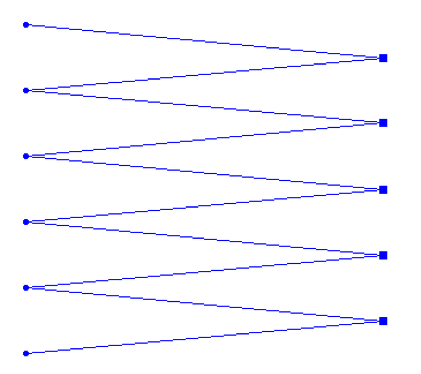
\includegraphics{images/BufferSize5.png}


We see five factors and 6 variables.  After the first time we call �advance�, BlastFromThePast factors will be added to the oldest variable.  These factors contain messages from the past. 
There are two ways to set the BufferSize for a FactorGraph stream:

\begin{itemize}
\item Fg.addFactor(ng,bufferSize,stream,slice,etc...); - Specified as second argument to addFactor.
\item Fgs = fg.addFactor(ng,stream,slice,etc...);
\ifmatlab
fgs.BufferSize = bufferSize; - Set on the FactorGraphStream directly.
\fi
\ifjava
fgs.setBufferSize(bufferSize); - Set on the FactorGraphStream directly.
\fi
\end{itemize}

\para{DataSources}

Users can create data sources and attach them to VariableStreams.  As variables are created, data is retrieved from the DataSources and applied as inputs to the variables.  If a VariableStream is never connected to a DataSource, hasNext() will always return true for that VariableStream.  When a VariableStream is connected to a data source, hasNext() only returns true when there's more data in the DataSource.

DataSources implement the hasNext and getNext methods.  Methods include:

\ifmatlab
\begin{itemize}
\item DoubleArrayDataSource(); -- Constructor that creates an empty data source
\item DoubleArrayDataSource(data); -- Constructor that expects a matrix as input.  The data should be formatted such that each column provides input data for a step in the rolled up graph.
\item DoubleArrayDataSource(dimensions); -- Dimensions is a row vector specifying the dimensions of the variable for each step of the repeated graph.
\item DoubleArrayDataSource(dimensions,data); -- Dimensions means the same as above.  The data is added to the double array data source as though add(data) were called.  See the following:
\item add(data); -- Users can add  more data to the end of the data source.  Data should have the following dimensions: [VarDimensions SizeOfInputData NumSteps).  So if the user creates an MxN variable and wants to repeat it P times and the variable has domain of length K, the data should have the dimensions: [M N K P]
\end{itemize}
\fi

\ifjava
\begin{itemize}
\item DoubleArrayDataSource(); -- Constructor that creates an empty data source
\item DoubleArrayDataSource(data); -- Constructor that expects a two dimensional array as input.  The data should be formatted such that each row provides input data for a step in the rolled up graph.
\item add(data); -- Users can add  more data to the end of the data source.  Data should have the following dimensions: NumSteps x SizeOfInputData.
\end{itemize}
\fi

Dimple also has support for MultivariateDataSources.

\ifmatlab
\begin{itemize}
\item MultivariateDataSource(); -- Creates a data source object and assumes there is a single variable per step.
\item MultivariateDataSource(dimensions) -- Creates a data source objects that can be associated with a variable stream with the given dimensions.
\item add(means,covariance) -- Means should be in the form [VarDimensions NumberMeansPerVar] and Covariance should be of the form [VarDimensions NumberMeansPerVar NumberMeansPerVar] 
\end{itemize}
\fi

\ifjava
\begin{itemize}
\item MultivariateDataSource(); -- Creates a data source object and assumes there is a single variable per step.
\item add(means,covariance) -- Means is the vector of means and covariance should contain a 2d array representing the covariance matrix.
\end{itemize}
\fi

\para{DataSink}

Users can retrieve their data using data sinks.

\ifmatlab
\begin{itemize}
\item DoubleArrayDataSink(); -- Create a double array data sink
\item DoubleArrayDataSink(dimensions) -- Creates a double array data sink for a variable with the specified dimensions.
\item MultivariateDataSink() -- Created a multivariate data sink
\item MultivariateDataSink(dimensions) -- Creates a multivariate data sink with the specified dimensions.
\item hasNext() -- Is there more data in the data sink?
\item getNext() -- Retrieve the next chunk of data.  For DoubleArrays, this returns data in the same form as is supplied to data sources.  The MultivariateDataSink object returns MultivariateMsg objects.
\item varStream.DataSink = dataSink; -- Data sinks can be assigned to variable streams.
\end{itemize}
\fi

\ifjava
\begin{itemize}
\item DoubleArrayDataSink(); -- Create a double array data sink
\item MultivariateDataSink() -- Created a multivariate data sink
\item hasNext() -- Is there more data in the data sink?
\item getNext() -- Retrieve the next chunk of data.  For DoubleArrays, this returns data in the same form as is supplied to data sources.  The MultivariateDataSink object returns MultivariateMsg objects.
\item varStream.setDataSink(dataSink); -- Data sinks can be assigned to variable streams.
\end{itemize}
\fi

\para{Accessing Variables}
In the absence of data sinks, users need a way to retrieve variables to get beliefs.   The following methods allow the user to do that:

\ifmatlab
\begin{lstlisting}
Vs = BitStream();
\end{lstlisting}

\begin{itemize}
\item Vs.Size -- Number of variables in the buffer.
\item Vs.get(index) -- Retrieves a variable of the specified index.  This is a 1-based value.
\end{itemize}
\fi

\ifjava
\begin{lstlisting}
BitStream Vs = new BitStream();
\end{lstlisting}

\begin{itemize}
\item Vs.setSize(size) -- Number of variables in the buffer.
\item Vs.get(index) -- Retrieves a variable of the specified index.  This is a 1-based value.
\end{itemize}

\fi

\subsubsection{Markov Model with Parameter}


When adding a repeated graph, it is possible to specify some variables as streams and others as individual variables.  We sometimes call these individual variables parameters.  Using this feature is straightforward:

\ifmatlab
\begin{lstlisting}
ng = FactorGraph(a,b);
ng.addFactor(@xorDelta,a,b);
p = Bit();
s = BitStream();
fg = FactorGraph();
fgs = fg.addFactor(ng,p,s);
fgs.BufferSize = 5;
fg.plot();
\end{lstlisting}
\fi

\ifjava
\begin{lstlisting}
Equals eq = new Equals();
FactorGraph ng = new FactorGraph(a,b);
ng.addFactor(eq,a,b);
Bit p = new Bit();
BitStream s = new BitStream();
FactorGraph fg = new FactorGraph();
FactorGraphStream fgs = fg.addRepeatedFactor(ng,p,s);
fgs.setBufferSize(5);
\end{lstlisting}
\fi


This code results in the following graph:

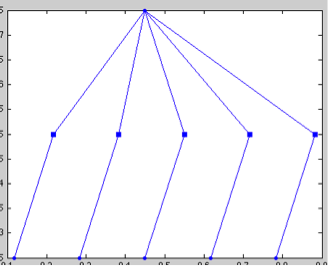
\includegraphics{images/RolledUpParameter.png}

\subsubsection{Real Variables}

Rolled up graphs work with real variables as well.  Here we create another Markov Model.  We use the Gaussian solver that supports a custom factor called �constmult�.  We create a data source that only has information about the first variable.  The means beliefs are growing by 110\% as we iterate through the stream because the factor provides a constraint that each variable is 110\% of the previous variable.

\ifmatlab
\begin{lstlisting}
%%%%%%%%%%%%%%%%%%%%%%%%%%%%%%                                                                                                
%Set solver type so we can create reals                                                                                       
%%%%%%%%%%%%%%%%%%%%%%%%%%%%%%                                                                                                
setSolver('Gaussian');

%%%%%%%%%%%%%%%%%%%%%%%%%%%%%%                                                                                                
%Build graph                                                                                                                  
%%%%%%%%%%%%%%%%%%%%%%%%%%%%%%                                                                                                
a = Real();
b = Real();

ng = FactorGraph(a,b);
ng.addFactor(@constmult,b,a,1.1);

fg = FactorGraph();
s = RealStream();

fg.addFactor(ng,s,s.getSlice(2));

%%%%%%%%%%%%%%%%%%%%%%%%%%%%%%                                                                                                
%set data                                                                                                                     
%%%%%%%%%%%%%%%%%%%%%%%%%%%%%%                                                                                                

data = [[1; .1] repmat([0 Inf]',1,10)];
dataSource = DoubleArrayDataSource(data);


s.DataSource = dataSource;
s.DataSink = DoubleArrayDataSink();

%%%%%%%%%%%%%%%%%%%%%%%%%%%%%%                                                                                                
%Solve                                                                                                                        
%%%%%%%%%%%%%%%%%%%%%%%%%%%%%%                                                                                                
fg.solve();


%%%%%%%%%%%%%%%%%%%%%%%%%%%%%%                                                                                                
%get belief                                                                                                                        
%%%%%%%%%%%%%%%%%%%%%%%%%%%%%%                                                                                                
while s.DataSink.hasNext();
    disp(s.DataSink.getNext());
end
\end{lstlisting}
\fi

\ifjava
\begin{lstlisting}
///////////////////////////////////////                                                                                                
//Set solver type so we can create reals                                                                                       
///////////////////////////////////////

Model.getInstance().setDefaultGraphFactory(new com.analog.lyric.dimple.solvers.gaussian.Solver());

///////////////////////////////////////                                                                                                
//Build graph                                                                                                                  
///////////////////////////////////////                                                                                                
Real a = new Real();
Real b = new Real();

FactorGraph ng =  new FactorGraph(a,b);
ng.addFactor(new NopFactorFunction("constmult"), b,a,1.1);

FactorGraph fg = new FactorGraph();
RealStream s = new RealStream();

fg.addRepeatedFactor(ng,s,s.getSlice(2));

///////////////////////////////////////                                                                                                
//set data                                                                                                                     
/////////////////////////////////////// 

double [][] data = new double[11][];
data[0] = new double [] {1,0.1};
for (int i = 1; i < 11; i++)
	data[i] = new double [] {0,Double.POSITIVE_INFINITY};

DoubleArrayDataSource dataSource = new DoubleArrayDataSource(data);

s.setDataSource(dataSource);
s.setDataSink(new DoubleArrayDataSink());


///////////////////////////////////////                                                                                                
//Solve                                                                                                                        
///////////////////////////////////////                                                                                                
fg.solve();

///////////////////////////////////////                                                                                                
//get belief                                                                                                                        
///////////////////////////////////////
DoubleArrayDataSink dds = (DoubleArrayDataSink)s.getDataSink();
while (dds.hasNext())
{			
	double [] tmp = dds.getNext();
    System.out.println(Arrays.toString(tmp));
}
\end{lstlisting}
\fi

This produces the following output:

\ifmatlab
\begin{lstlisting}
    1.0000    0.1000

    1.1000    0.1100

    1.2100    0.1210

    1.3310    0.1331

    1.4641    0.1464

    1.6105    0.1611

    1.7716    0.1772

    1.9487    0.1949

    2.1436    0.2144
\end{lstlisting}
\fi

\ifjava
\begin{lstlisting}
[1.0, 0.1]
[1.1, 0.11000000000000001]
[1.2100000000000002, 0.12100000000000002]
[1.3310000000000004, 0.13310000000000002]
[1.4641000000000006, 0.14641000000000004]
[1.6105100000000008, 0.16105100000000006]
[1.771561000000001, 0.17715610000000007]
[1.9487171000000014, 0.1948717100000001]
\end{lstlisting}
\fi


\subsubsection{Manually Advancing}
\label{sec:manuallyAdvancingRolledUpGraph}

By default, rolled up graphs will advance until there is no data left in a DataSource.  Users may override this behavior by either using FactorGraph.solveOneStep or setting the FactorGraph.NumSteps parameter.  By default, NumSteps is set to Inf.  By setting this to a finite number, N, users can examine the graph at every N steps of the rolled up graph.  This allows the user to pull Beliefs off of any portion of the graph.

\ifmatlab
\begin{lstlisting}
%%%%%%%%%%%%%%%%%%%%%%%%%%%%%%%%%%%%%%%%%%%%
%simple Markov Model with larger buffer size

%Create the data
N = 10;
data = repmat([.4 .6]',1,N);

%Create a data source
dataSource = DoubleArrayDataSource(data);

%Create a variable stream.
vs = DiscreteStream({0,1});
vs.DataSource = dataSource;

%Create our nested graph
in = Bit();
out = Bit();
ng = FactorGraph(in,out);
ng.addFactor(@(a,b) a==b,in,out);

%Create our main factor graph
fg = FactorGraph();

%Build the repeated graph
bufferSize = 2;
fgs = fg.addFactor(ng, bufferSize, vs,vs.getSlice(2));

%Initialize our messages
fg.initialize();

while 1
    %Solve the current time step
    fg.solveOneStep();
    
    %Get the belief for the first variable
    belief = vs.get(3).Belief;
    disp(belief)

    if fg.hasNext
        fg.advance();
    else
        break;
    end
end
\end{lstlisting}
\fi

\ifjava
\begin{lstlisting}
//simple Markov Model with larger buffer size
Equals eq = new Equals();

//Create the data
int N = 10;
double [][] data = new double[N][];
for (int i = 0; i < N; i++)
	data[i] = new double [] {0.4,0.6};

//Create a data source
DoubleArrayDataSource dataSource = new DoubleArrayDataSource(data);

//Create a variable stream.
DiscreteStream vs = new DiscreteStream(0,1);
vs.setDataSource(dataSource);

//Create our nested graph
Bit in = new Bit();
Bit out = new Bit();
FactorGraph ng = new FactorGraph(in,out);
ng.addFactor(eq,in,out);

//Create our main factor graph
FactorGraph fg = new FactorGraph();

//Build the repeated graph
int bufferSize = 2;
FactorGraphStream fgs = fg.addRepeatedFactorWithBufferSize(ng, 
		bufferSize,vs,vs.getSlice(2));


//Initialize our messages
fg.initialize();

while (true)
{
    //Solve the current time step
    fg.solveOneStep();
    
    //Get the belief for the first variable
    double [] belief = ((double[])vs.get(2).getBeliefObject());
    		System.out.println(Arrays.toString(belief));

    if (fg.hasNext())
    	fg.advance();
    else
    	break;
}
\end{lstlisting}
\fi

In this code snippet, the user initializes the graph and calls advance until there is no data left.  At each step, the user retrieves the beliefs from the third instance of the variable in the variable stream.

The user can also progress N steps:

\ifmatlab
\begin{lstlisting}
%Initialize our messages
fg.initialize();
fg.NumSteps = 2;

while 1
    %Solve the current time step
    fg.continueSolve(); %This method is need to avoid initialization
    
    %Get the belief for the first variable
    belief = vs.get(3).Belief;
    disp(belief)

    if fg.hasNext
        fg.advance();
    else
        break;
    end
end
\end{lstlisting}
\fi

\ifjava
\begin{lstlisting}
//Initialize our messages
fg.initialize();
fg.setNumSteps(2);

while (true)
{
    //Solve the current time step
    fg.continueSolve(); //This method is need to avoid initialization
    
    //Get the belief for the first variable
    //Get the belief for the first variable
    double [] belief = ((double[])vs.get(2).getBeliefObject());
    		System.out.println(Arrays.toString(belief));

    if (fg.hasNext())
    	fg.advance();
    else
    	break;
}

\end{lstlisting}
\fi

